
\section{Supplementary material}
\label{sec:supp}

 (e.g., relative difference, log-RMSE, etc.) are RMSE variations commonly used for evaluation of depth SR methods.
 
 
 CNN-based approaches to visual simuilarity proved to be efficient in the context of texture synthesis
\cite{gatys2015texture,lu2016learning}. 

In \cite{chen2018single} they consider single depth image super-resolution. First, an edge-map from low-res depth is acquired using CNN. Then an empirical edge map refinement is applied together with the edge-guided depth upsampling. This approach requires construction of the labeled sample for CNN edge detector training. The author used canny edge detector which provides noisy labels and so the resulting CNN edge detector is not reliable. Another approach to single depth image super-resolution with large up-sampling factors is described in \cite{song2018deeply}. The idea is to represent the task of depth map super-resolution as a series of novel view synthesis sub-tasks and apply a deeply supervised network to generate a depth map from different camera pose and then to perform a multi-scale fusion strategy to exploit the feature maps at different scales and obtain a final result. However, the approach looks sensitive \EB{maybe say something more objective?} to distortions of pixels on borders, occurring when generating depth maps from different camera poses. 


\cite{lu2015sparse} develop a filtering-based framework for depth upsampling from extremely low-resolution input such as $64 \times 64$ pixels, achieving impressive results for upsampling factors as large as $\times 64$. 

Other methods aimed directly at the surface reconstruction could be mentioned (cf.~\cite{haque2017multi,maier2017intrinsic3d,zuo2017detailed}), yet they require a sequence of RGB-D images as an input. In contrast, we only consider single-image RGB-D input. Additionally, these methods directly optimize the surface reconstruction target, while, in our setup, we only evaluate against a proxy functional related to visual surface quality. 

In \cite{kim2018deformable}, the authors propose a linear filtering model for depth SR, but with non-linear kernel based on CNN architecture that outputs set of neighbours and their corresponding weights adaptively for each pixel.  \cite{agresti2017deep} proposes a framework for the fusion of depth data produced by ToF camera and a stereo vision system by utilising confidence maps for both sources using a CNN architecture. \cite{zhao2017simultaneously} considers a modification of the generative adversarial networks that given low-resolution depth and color images leverages mutual information to enhance each other and provide depth SR. Adversarial loss is used only for color images to make them more realistic. Thus, we can simultaneously perform depth-color SR. However, in practice it is a rare situation when a color image has the same resolution as a depth image, usually we acquire color images in higher resolution.

\cite{jiang2018depth} formulates an optimization approach and proposes an autoregressive model to explore the high-order correlations of sparse codes. Similarly, \cite{ham2018robust} present an optimization-based filtering method where the weighted data fidelity term is balanced against a non-convex regularizer. \cite{yang2014color} proposes an autoregressive regularizer $R(I) = E_{AR}(I)$ and a structure-aware filter to define its parameters. As opposed to such approaches, which require custom hand-crafted regularizers and optimization procedures, our CNN-based methods are fully learnable using a standard computational framework of deep learning (e.g. gradient-based optimization), in particular, we employ an off-the-shelf network architecture and optimizer. 

In \cite{zuo2018minimum} the guided depth map super-resolution based on a novel Markov Random Field model is proposed. Here the guidance from the high-quality color image uses the special distance between pixels in a space consisting of the minimum spanning trees (forest) to better preserve depth edges. A number of additional tricks such as usage of the explicit edge inconsistency measurement model to reduce texture-copying artifacts. However, the model is overwhelmingly complex due a nested structure of regularisation terms with various weights, which are some complex functionals of the lwo-resolution depth maps in their turn. Moreover, for each new type of images a number of hyperparameters (e.g. the threshold in Huber loss, the regularisation coefficient in the MRF model loss, the bandwidth for the kernel based on the Minimum Spanning Forest, the number of super-pixels) should be tuned anew, which is not possible in the wild.



\section{Methods}
\label{sec:_methods}

% Motivation:
% 1. We're using surface-(geometry-)aware loss/metrics to (1) evaluate how good is the reconstruction, (2) do visually better on reconstruction
% 2. We have selected a number of approaches known from literature (describe them here). 
% 3. This is how we performed this selection: (1), (2), (3).
% 3. This is the summary of the compared approaches.
% 4. This is the descriptions of the approaches themselves. Here is the minimized metric, and other stuff that's interesting about them.
% 5. We propose our methods: here are their descriptions.

The  intuition behind our evaluation is to abstract from the original problem and method architecture, concentrating on the assessment of the visual quality of the resulting 3D surface. We question whether RMSE provides a good measure of the visual quality of the result produced by an original method. 
% Targeting the assessment of visual reconstruction quality, we form a representative set of recent approaches to single-image depth super-resolution, that we compare with our proposed method. 
Note that we don't aim for an exhaustive evaluation of the available approaches or for a comprehensive comparison with state-of-the-art, but rather focus on comparing against a possibly broader range of competitors. 
We selected 8 range-image handling methods with distinct underlying principles: deep CNN-based \cite{riegler2016deep,hui2016depth,mal2018sparse,yan2018ddrnet,Ulyanov_2018_CVPR} 
and non-CNN-based \cite{gu2017learning} learnable methods,
optimization-based \cite{haefner2018fight},
and filtering-based approaches \cite{xie2016edge}. 
On the application side, they correspond to a variety of target tasks 
such as regular super-resolution~\cite{riegler2016deep,hui2016depth,haefner2018fight,xie2016edge},
denoising~\cite{yan2018ddrnet,gu2017learning}, and 
densification~\cite{mal2018sparse} of depth images, with~\cite{Ulyanov_2018_CVPR} focusing on the super-resolution of photos. 
We omit the comparison with some methods (such as~\cite{zhang2018image}), even though they report state-of-the-art results. 
In this section, we give details describing our choice of the competitor models from the literature and present our novel approach.
% \todo{basically the idea here would be that no matter what method and which task it was originally trained on, perceptual metrics show how good the result is in terms of the perceived quality of the surface}

% The selection was performed according to the following criteria: (1) availability of code used for testing the model, (2) only post-2014 methods were considered. \LA{how else did we select?}
% We validate our evaluation methodology using a broad range of recent approaches to single-image depth super-resolution. 
% As the evaluated methods, we have selected a number of recent approaches to single image depth super-resolution. 
% \todo{add motivation for evaluating these methods? why is this interesting? how is each method important for our work?}

\paragraph{The evaluated methods.} 
\noindent\emph{Deep multi-scale guided networks \cite{hui2016depth}.} 
A representative, carefully-designed and state-of-the-art deep learning architecture, MSG-Net upsamples different spectral components of $\lowresdepth$ (\eg, high-frequency \vs.\ low-frequency components) using different strategies. The upsampling is done in two learnable branches -- one for an intensity component, performing spatial downsampling, and another for a depth component, performing spatial downsampling, which fuse the feature maps obtained at equal spatial resolutions. The model is trained by minimizing the MSE on the training set. In our evaluation, we fully re-implement the method in our PyTorch code.

\noindent\emph{Deep primal-dual networks \cite{riegler2016deep}.}
Standing out of the typical mostly empirical approaches, the state-of-the-art PDN model features two stages: the first is composed of fully-convolutional layers that produce a rough super-resolved depth $\widehat{d}^{\mathrm{(HR)}} = \mathsf{fcn}(\lowresdepth, \hiresimage)$, and the second solves an unrolled variational optimization problem that estimates sharp and noise-free results. The model is optimized in an end-to-end fashion by simultaneously training parameters of convolutional layers and solving a variational optimization problem:
\[
\widehat{d}^{\mathrm{(HR)}}_* = 
    \argmin\limits_{d} \mathcal{E}_{\mathrm{MSE}}(d, \mathsf{fcn}(\lowresdepth, \hiresimage)) 
    + \lambda \mathcal{R}(d),
\]
with $\mathcal{R}(d)$ providing a non-local Huber regularization to the solution via a custom weighting of the Huber norm. To run the method, we use the publicly available LuaTorch implementation\footnote{\url{https://github.com/griegler/primal-dual-networks}}.

\noindent\emph{Learnable dynamic guidance~\cite{gu2017learning}} is a state-of-the-art depth image enhancement method, which produces a solution to the following bi-level optimization problem:
\begin{multline}
\{\rho^*_l, \bm{\beta}^*_l, \bm{k}^*_l\}_{l=1}^L = 
    \argmin\limits_{\{\rho_l, \bm{\beta}_l, \bm{k}_l\}_{l=1}^L}
    \sum\limits_{s = 1}^S \| \hiresdepthest_s - \hiresdepth_s \|_2^2\\
\mbox{\textit{s.t.}} \quad \hiresdepthest_s = 
    \argmin\limits_{d} \mathcal{E}_{\mathrm{MSE}}(d, \lowresdepth_s) \\
    + \sum\limits_l \sum\limits_i w_{l,i}(\hiresimage_s) \rho_l( (\bm{k}_l * d)_i ),
\end{multline}
where $w_{l,i}(\hiresimage_s)$ is a parametrized weight function controlling the relative influence of low-resolution depth $\lowresdepth_s$ and high-resolution image $\hiresimage_s$ on the output $\hiresdepth_s$, $\{\bm{k}_l\}_{l=1}^L$ is a collection of convolutional filters, and $\{\rho_l\}_{l=1}^L$ is a collection of parametrized penalty functions serving as a regularizer. We use the publicly available MATLAB code\footnote{\url{https://sites.google.com/site/shuhanggu/home}}.

\noindent\emph{Depth super-resolution from shading~\cite{haefner2018fight}} is a state-of-the-art depth super-resolution method using shape-from-shading optimization. The method bases on an insight that high-frequency information necessary to achieve depth super-resolution which preserves details could be provided by the photometric data. Similarly, the low-frequency information necessary to disambiguate shape-from-shading could be conveyed by the geometric data. They achieve joint depth map refinement and super-resolution in a single shot, without resorting to extra data such as additional viewing angles or information on illumination conditions. The method is formulated in Bayesian terms as a variational problem minimizing a weighted multi-task objective function including shape priors, surface albedo, lighting model, and MSE-based data fidelity terms. We use a MATLAB implementation of this method shared with us by the authors.

% Because of that some information is added with priors for shape of object, albedo function of the surface, lighting model and even the choice of basis functions for prior representation.

\noindent\emph{Edge-guided depth super-resolution~\cite{xie2016edge}} is a state-of-the-art depth-only MRF-based super-resolution approach combining depth upsamping with high resolution smooth edge prediction problem. As edges are of particular importance in the texture-less depth image, such a guidance method can alleviate blurring artifacts around edges, which get generated by direct depth value prediction. The method works by first predicting a high resolution edge map, followed by interpolation and smoothing of the high resolution depth textures with a modified joint bilateral filter. We use the publicly available MATLAB code\footnote{\url{https://github.com/ClaireXie/edgeGuidedSDSP}}.

% Color assisted joint up-sampling approach - in which the high resolution color image provides the edge information to pixels in a local region with different depth, so that they could be weighted in the up-sampling process.

% Although reconstruction is guided by the edge map, the high resolution depth image will still contain defects inside the edge boundary.

\noindent\emph{Deep sparse-to-dense regression networks~\cite{mal2018sparse}}, a state-of-the-art densification representative CNN, considers problem of dense depth prediction from a sparse set of depth measurements and a single RGB image. In our interpretation, $\lowresdepth$ could serve as such a sparse (but regular) set of depth measurements, transforming the problem to depth super-resolution. The method works by a direct minimization of the Huber loss via an deep encoder-decoder CNN. We use the publicly available PyTorch implementation\footnote{\url{https://github.com/fangchangma/sparse-to-dense}}.

\noindent\emph{Deep denoising and refinement networks~\cite{yan2018ddrnet}.}
The model proceeds in two stages. First, denoise the input low-resolution depth image $\lowresdepth$ using an encoder-decoder CNN, trained to minimize a weighted sum of per-pixel mean absolute error (MAE), MSE, and normal-derived terms. Second, the denoised depth map is refined with high-frequency details by passing it through a CNN, along with an accompanying high-resolution RGB image $\hiresimage$. A peculiar property of the refinement network is that it explicitly minimizes MSE difference of reflected irradiance between the prediction $\hiresdepthest$ and the ground truth $\hiresdepth$, bearing some similarity to our perceptually-based metrics.

\noindent\emph{Deep image prior~\cite{Ulyanov_2018_CVPR}} is a state-of-the-art image super-resolution representative based on a remarkable observation, that the structure of the network itself, without any specialized training, may be used for optimization, resulting in a zero-shot upsampling method. DIP uses a deep fully-convolutional model to solve for
\[
\widehat{d}^{\mathrm{(HR)}}_* = 
    \argmin\limits_{d} \mathcal{E}_{\mathrm{MSE}}(\mathrm{CNN}(z; \theta), \lowresdepth)
\]
where the minimizer $\widehat{d}^{\mathrm{(HR)}}_*$ is anything that a neural net $\mathrm{CNN}(z; \theta)$ was able to produce from a random tensor $z$. We note that such a model is mask/hole-agnostic and allows for simultaneous super-resolution\,\&\,enhancement without any modifications. We use the publicly available and official PyTorch implementation\footnote{\url{https://github.com/DmitryUlyanov/deep-image-prior}}.

We note that all methods (except for~\cite{xie2016edge}) use high-resolution RGB guidance image as additional input. Interestingly, neither of the methods (except for~\cite{yan2018ddrnet} which adds a normal-derived loss as a proxy to the surface) was trained to output a high-quality surface.

\paragraph{Our methods.} 

\begin{multline*}
\widehat{d}^{\mathrm{(HR)}}_* = 
    \argmin\limits_{d} \mathcal{E}_{\mathrm{MSE}}(d, \hiresdepth) +
    \mathcal{E}_{\mathrm{SURF}}(d, \hiresdepth) 
\end{multline*}

We choose 
\begin{multline}
\label{eq:supp_our_visual_metric}
\widehat{d}^{\mathrm{(HR)}}_* = 
    \argmin\limits_{d} \mathcal{E}_{\mathrm{LAP}}(d, \hiresdepth) +
    \mathcal{E}_{\mathrm{SIN}}(d, \hiresdepth) 
\end{multline}





\begingroup
\setlength{\tabcolsep}{2pt} % Default value: 6pt
\renewcommand{\arraystretch}{0} % Default value: 1

\begin{figure*}[t]
\captionsetup[subfigure]{labelformat=empty}
\begin{center}

\begin{tabular}{cccccccc}
\subfloat{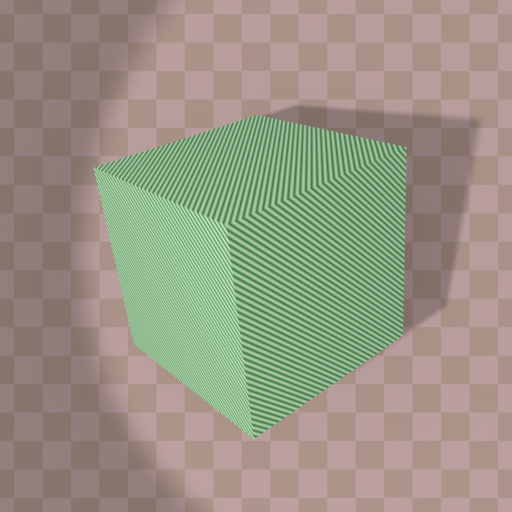
\includegraphics[width = 2cm]{img/simgeo.cube_on_plane.textured.rgb.png}} &
\subfloat{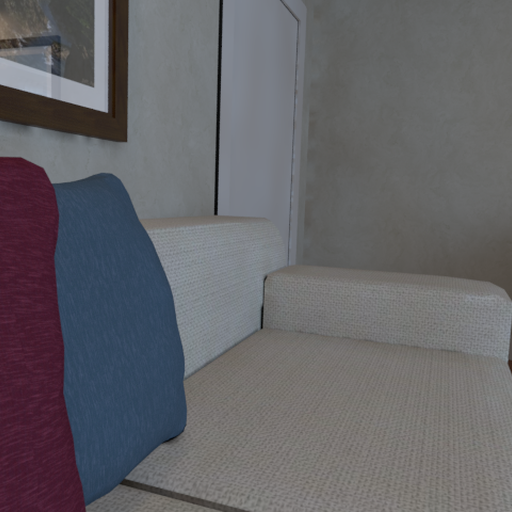
\includegraphics[width = 2cm]{img/icl-nuim.living.rgb.png}} &
\subfloat{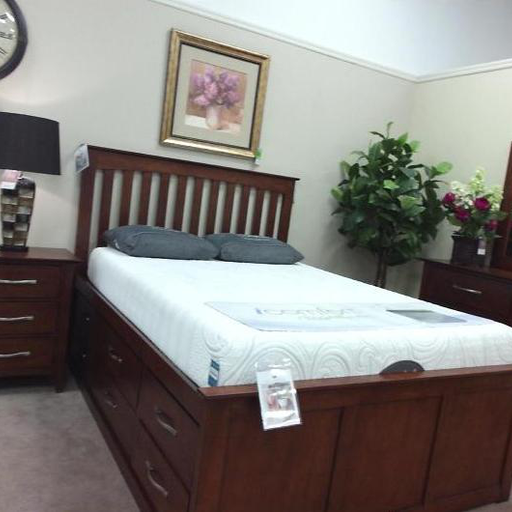
\includegraphics[width = 2cm]{img/sun-rgbd.kv2.rgb.png}} &
\subfloat{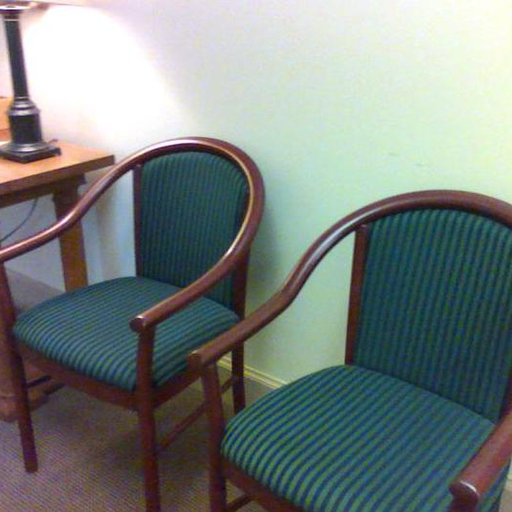
\includegraphics[width = 2cm]{img/sun-rgbd.realsense.rgb.png}} &
\subfloat{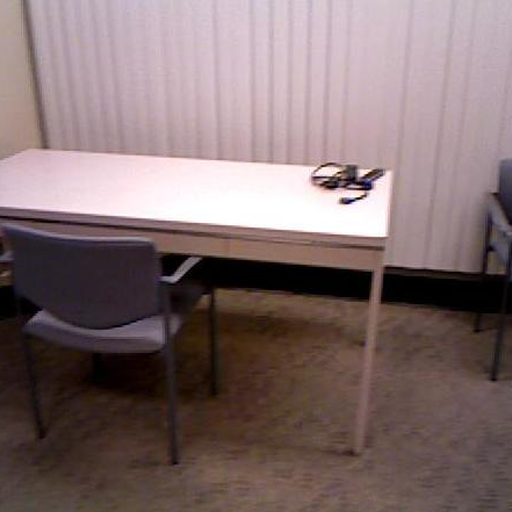
\includegraphics[width = 2cm]{img/sun-rgbd.xtion.rgb.png}} &
\subfloat{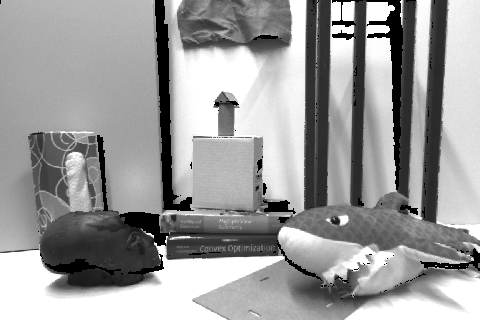
\includegraphics[width = 2cm]{img/tofmark.shark.rgb.png}} &
\subfloat{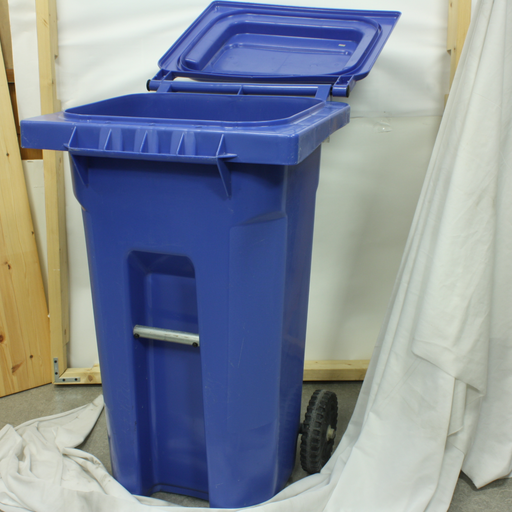
\includegraphics[width = 2cm]{img/middlebury.simple.recycle.rgb.png}} &
\subfloat{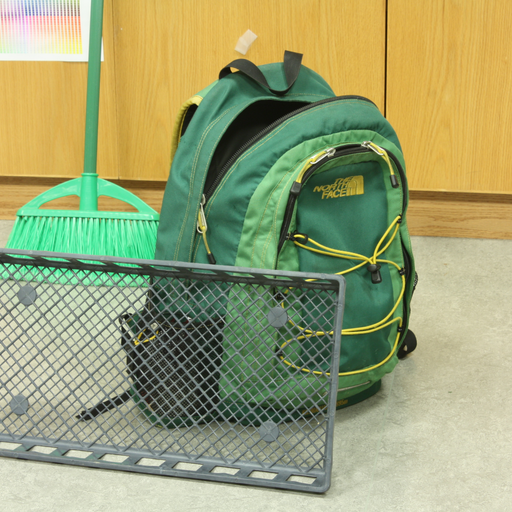
\includegraphics[width = 2cm]{img/middlebury.complex.backpack.rgb.png}} \\[0ex]
\subfloat{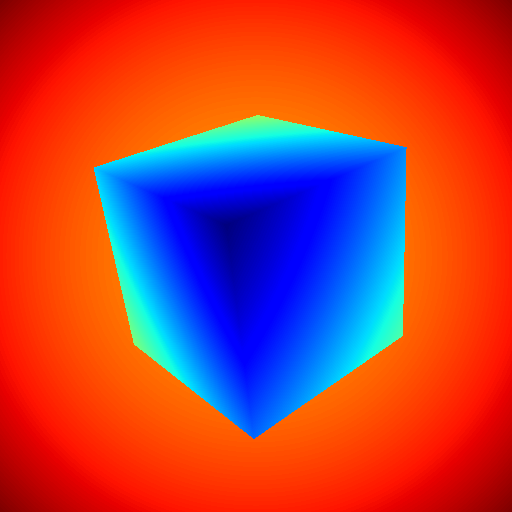
\includegraphics[width = 2cm]{img/simgeo.cube_on_plane.textured.depth.png}} &
\subfloat{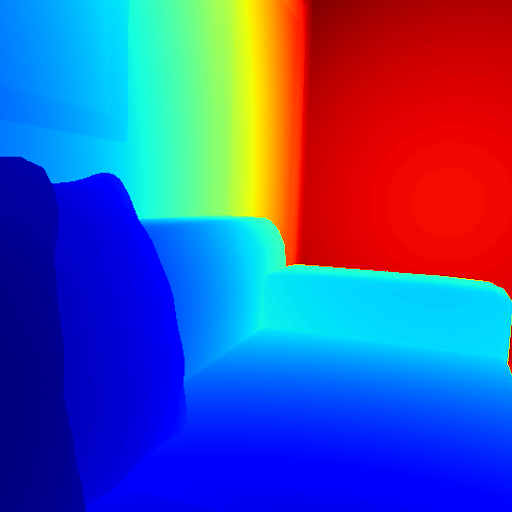
\includegraphics[width = 2cm]{img/icl-nuim.living.depth.png}} &
\subfloat{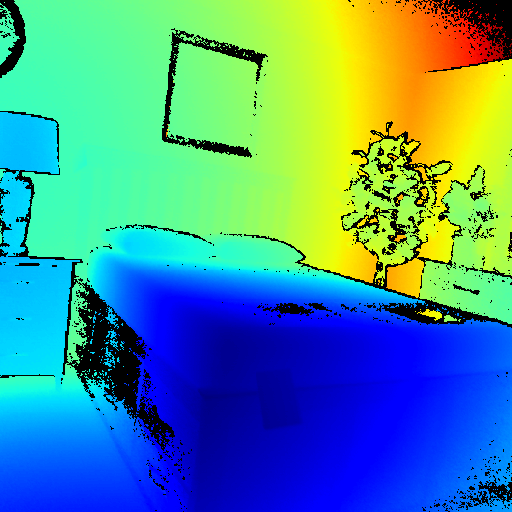
\includegraphics[width = 2cm]{img/sun-rgbd.kv2.depth.png}} &
\subfloat{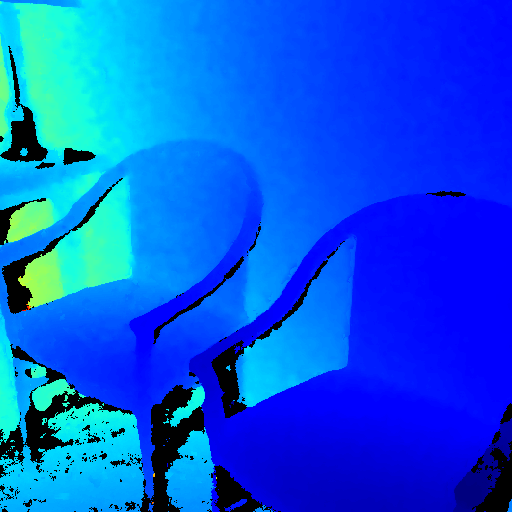
\includegraphics[width = 2cm]{img/sun-rgbd.realsense.depth.png}} &
\subfloat{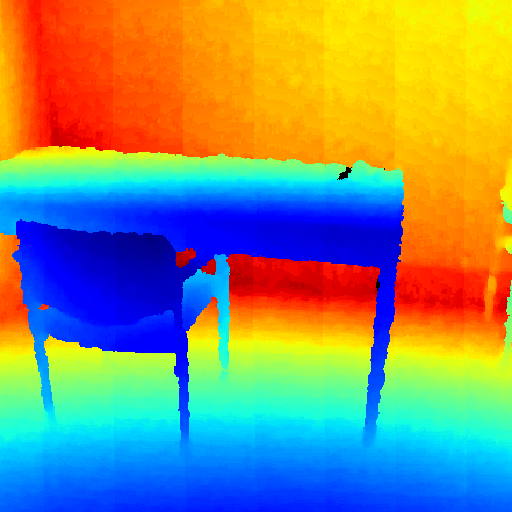
\includegraphics[width = 2cm]{img/sun-rgbd.xtion.depth.png}} &
\subfloat{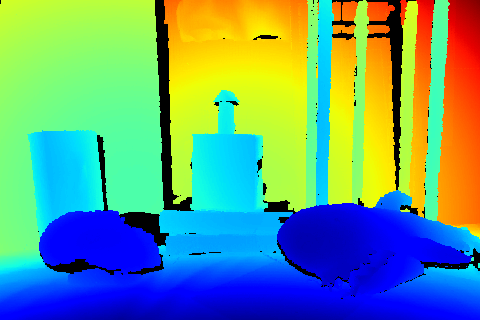
\includegraphics[width = 2cm]{img/tofmark.shark.depth.png}} &
\subfloat{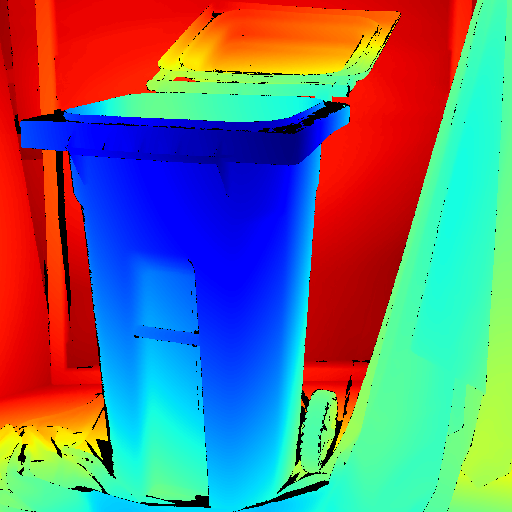
\includegraphics[width = 2cm]{img/middlebury.simple.recycle.depth.png}} &
\subfloat{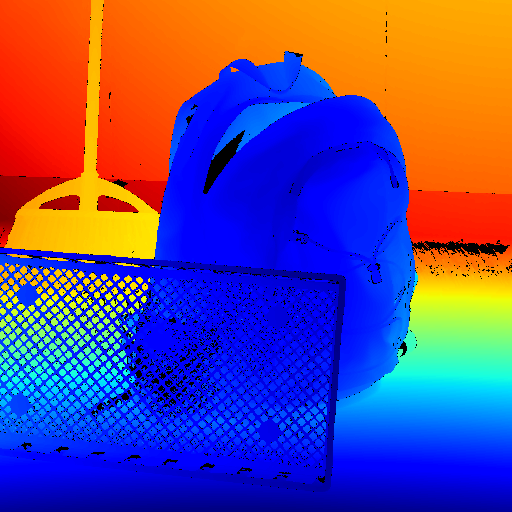
\includegraphics[width = 2cm]{img/middlebury.complex.backpack.depth.png}} \\[0ex]
\subfloat[\emph{SimGeo}]{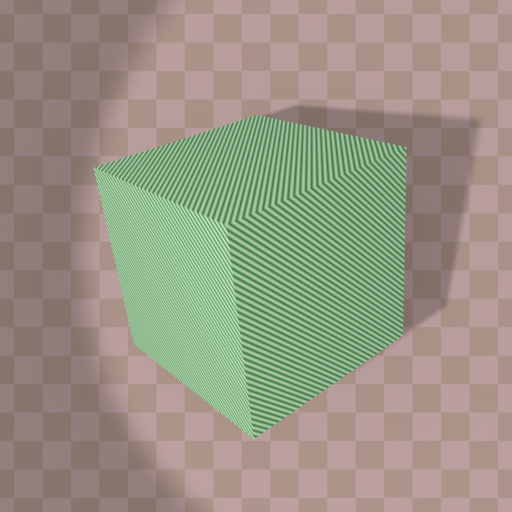
\includegraphics[width = 2cm]{img/simgeo.cube_on_plane.textured.rgb.png}} &
\subfloat[\emph{ICL-NUIM}]{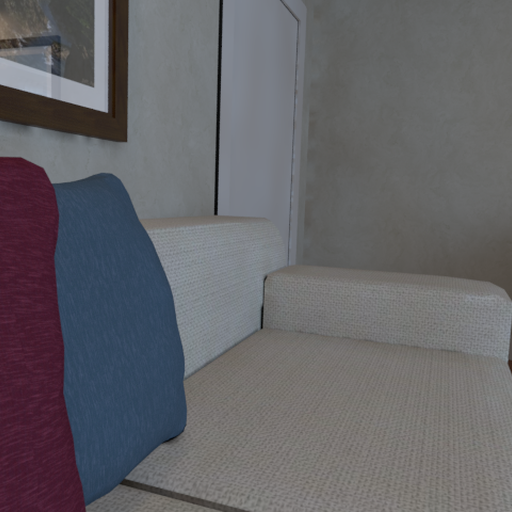
\includegraphics[width = 2cm]{img/icl-nuim.living.rgb.png}} &
\subfloat[\emph{KinectV2}]{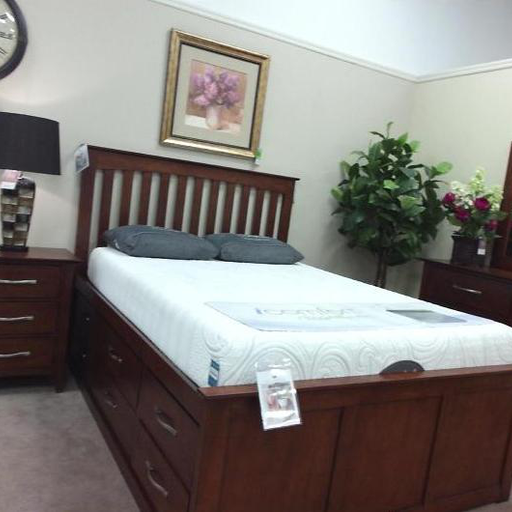
\includegraphics[width = 2cm]{img/sun-rgbd.kv2.rgb.png}} &
\subfloat[\emph{RealSense}]{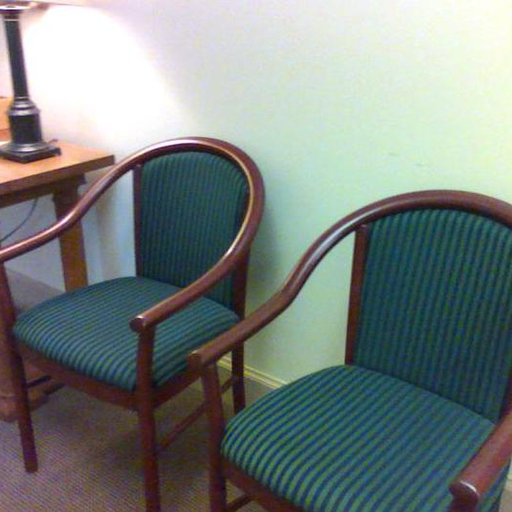
\includegraphics[width = 2cm]{img/sun-rgbd.realsense.rgb.png}} &
\subfloat[\emph{Xtion}]{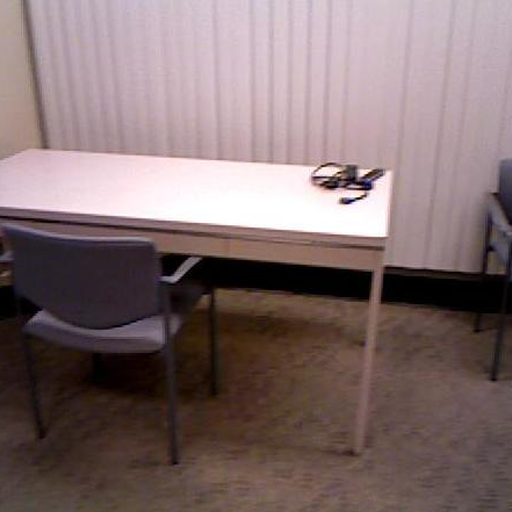
\includegraphics[width = 2cm]{img/sun-rgbd.xtion.rgb.png}} &
\subfloat[\emph{ToFMark}]{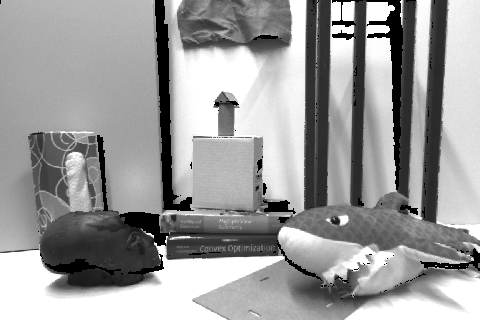
\includegraphics[width = 2cm]{img/tofmark.shark.rgb.png}} &
\subfloat[\emph{Simple}]{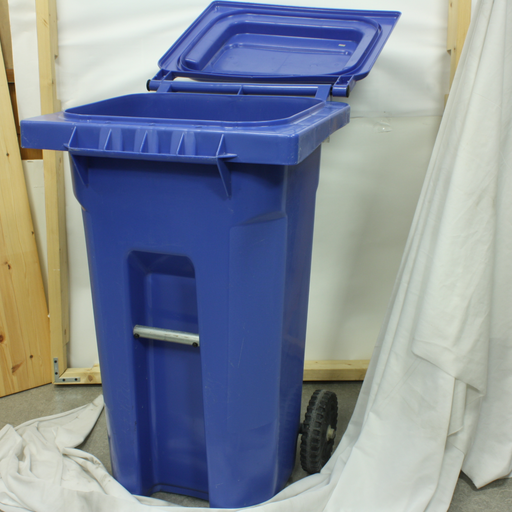
\includegraphics[width = 2cm]{img/middlebury.simple.recycle.rgb.png}} &
\subfloat[\emph{Complex}]{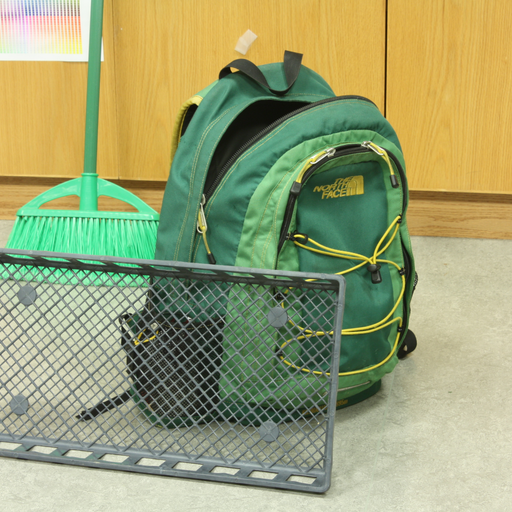
\includegraphics[width = 2cm]{img/middlebury.complex.backpack.rgb.png}} \\
\end{tabular}
\caption{Example images from our evaluation datasets corresponding to 8 categories. \todo{Add datasets images}}
\label{fig:supp_datasets}
\end{center}
\end{figure*}
\endgroup
% The \begingroup ... \endgroup pair ensures the separation
% parameters only affect this particular table, and not any
% sebsequent ones in the document.




% Characteristics for a dataset
% synthetic or real-world?
% which ground-truth data modality? (HQ/LQ result will be available)
% is extra highly-detailed?
% which sensor?
% original dataset?

\begin{table}
\begin{center}
\begin{tabular}{lllrr}
\toprule
Dataset                         & GT                & Sensor & 
\rotatebox[origin=c]{90}{Fine detail} & \rotatebox[origin=c]{90}{Real}\\
\midrule
Our \quad \emph{SimGeo}         & CAD               & render &          &       \\
\midrule
ICL-NUIM~\cite{handa:etal:ICRA2014}
                                & CAD               & render &          &       \\
\midrule
\multicolumn{5}{l}{SUN RGB-D~\cite{song2015sun}} \\
\quad \emph{KinectV2}           & time-of-flight    & time-of-fligh     &          &   \cm \\
\quad \emph{RealSense}          & structured light  & structured light  &          &   \cm \\
\quad \emph{Xtion}              & structured light  & structured light  &          &   \cm \\
\midrule
ToFMark~\cite{ferstl2013image}  & structured light  & time-of-flight &          &   \cm \\
\midrule
\multicolumn{5}{l}{Middlebury 2014~\cite{scharstein2014high}} \\
\quad \emph{Simple}             & structured light  & stereo &          &   \cm \\
\quad \emph{Complex}            & structured light  & stereo & \cm      &   \cm \\
\bottomrule
\end{tabular}
\end{center}
\caption{Overview of collected datasets and their capabilities.}
\label{tab:supp_datasets}
\end{table}


\OV{Provide example renderings from every part of our dataset}
